\section{A filling criterion and progressive characters}\label{sec:01-filling}

This section separates the geometric and algebraic ingredients of the filling
criterion.  The geometric ingredient preserves a prescribed finite part of a
filling kernel in a virtually compact special quotient of a finite-index
subgroup.  The algebraic ingredient uses these quotients to resolve the
coefficient problems left by an RFRS chain.

We specify the division-ring hypotheses, rather than assume that local
indicability alone supplies them.  For a group \(J\), write \(D(J)\) for a
division ring containing \(\Q J\).  Throughout this section the rings for
subgroups are compatible division closures inside the ambient ring; distinct
subgroup cosets are linearly independent over the corresponding subgroup
division ring; and finite-index coset representatives span the ambient
division ring over the subgroup division ring.  We also use the following
character consequence of Hughes-freeness.  If \(N=\ker\chi\), where \(\chi\)
is a real character of a finitely generated subgroup \(J\), then
\begin{equation}
 D(J)=\operatorname{Ore}\bigl(D(N)*(J/N)\bigr).
 \label{fill:field}
\end{equation}
Here the crossed product is embedded using coset representatives.  Its
quotient \(J/N\) is finitely generated free abelian, so the crossed product is
a Noetherian skew Laurent domain.  These are the subgroup-field properties
of the Hughes-free Linnell fields used in our applications; see
\cite{Hughes1970,Linnell1993} for their origins and
\cite[Corollaries~6.2--6.3]{JaikinLopezAlvarez2020} and
\cite[Section~2.3 and Proposition~2.2]{JaikinUniversality2021} for the
locally indicable affiliated realization and the normal-subgroup
crossed-product assertions. Arbitrary subgroup coset independence is
justified separately at the start of Section~\ref{sec:04-coefficients}.
We refer to this collection of properties as
the \emph{subgroup-field hypotheses}.

\begin{theorem}[Filling criterion]\label{fill:criterion}
Let \(G_*\) be a torsion-free hyperbolic group satisfying the following
conditions.
\begin{enumerate}[label=\textup{(\roman*)}]
\item \(G_*\) is locally indicable, coherent, of type \(F\), and has integral
cohomological dimension at most two.
\item \(G_*\) has a division ring \(D(G_*)\) satisfying the subgroup-field
hypotheses, and the chains of a finite classifying space become acyclic over
\(D(G_*)\).
\item There is a finite malnormal family \(\{D_j\}\) of quasiconvex
hyperbolic virtually compact special subgroups such that arbitrarily deep
peripheral fillings
\[
 G_*\longrightarrow Q_*
\]
are hyperbolic and virtually compact special, and their inherited peripheral
images are hyperbolic and virtually compact special.
\end{enumerate}
In \textup{(iii)}, arbitrarily deep means that the peripheral kernels can
avoid any prescribed finite subset of
\(\bigcup_j(D_j\setminus\{1\})\); the inherited peripheral structure is the
one furnished by relative Dehn filling.

Then a finite-index subgroup of \(G_*\) is an extension of a finite-rank free
group by \(\Z\).  Consequently \(G_*\) is virtually compact special.
\end{theorem}

The last conclusion uses cubulation of hyperbolic free-by-cyclic groups
\cite{HagenWise2016} and Agol's theorem \cite{Agol2013}.  We prove the other
conclusions below.  In particular, the original peripheral images in
Theorem~\ref{fill:criterion} need not be finite.

\subsection{Cofinite fillings and selective quotients}

Discard trivial members of the peripheral family. If no members remain,
the good filling is the identity, so hypothesis (iii) already says that
\(G_*\) is VCS. The same conclusion follows directly from (iii) if a
member equals \(G_*\). In these cases the RFRS argument at the end of the
section gives the stronger finite-rank free-by-\(\Z\) conclusion without
a geometric filling construction. Until then, assume all peripherals
are nontrivial proper subgroups.

By malnormal quasiconvex peripheralization, the pair
\((G_*,\{D_j\})\) is relatively hyperbolic
\cite{Bowditch2012,Osin2006}.  Suppose a sufficiently deep good filling as in
Theorem~\ref{fill:criterion}(iii) has been chosen, written
$q:G_*\to Q$. Choose this first filling to preserve every nonidentity
element of the total prescribed original finite list. Its peripheral
images $P_j=q(D_j)$ form an almost malnormal quasiconvex family in the
hyperbolic VCS group $Q$. The malnormal special quotient theorem supplies
designated finite-index normal subgroups $\dot P_j\unlhd P_j$
\cite[Theorem~2.7 and Corollary~2.8]{AGM2016}.

Each $P_j$ is residually finite. Choose finite-index normal subgroups
$L_j\unlhd P_j$ avoiding the finitely many nontrivial images that must
survive, as well as the additional relative-filling exclusions. Put
$M_j=\dot P_j\cap L_j$ and $R_j=(q|_{D_j})^{-1}(M_j)$.
Thus $M_j$ meets the designated containment condition, and the composite
quotient is exactly the filling by the normal finite-index $R_j$.
It is hyperbolic VCS by the special quotient theorem, with exact
peripheral images by relative filling. A finite $P_j$ allows $M_j=1$.
Thus we may, and do, choose a
cofinite good filling
\begin{equation}
 K=\langle\!\langle R_j:j\rangle\!\rangle_{G_*},
 \qquad Q_*=G_*/K,\qquad \bar D_j=D_j/R_j.
 \label{fill:cofinite}
\end{equation}
Every depth requirement below can be imposed before this choice.

For sufficiently deep fillings, the Cohen--Lyndon theorem
\cite[Definition~3.13 and Theorem~5.1]{Sun2020} identifies \(K\) with a free product
\begin{equation}
 K=\mathop{*}_{a\in\mathcal A} R_a,
 \label{fill:CL}
\end{equation}
where \(\mathcal A=\coprod_j Q_*/\bar D_j\) is the set of peripheral apex
images, and \(R_a\) is a suitably conjugated copy of \(R_j\).
The action of \(G_*\) permutes the conjugacy classes of these factors.
There are two coset sets here. Original peripheral cosets \(G_*/D_j\)
carry the conjugate rotation subgroups, whereas \(Q_*/\bar D_j\)
indexes their images after filling. All original apices over one
quotient apex form a \(K\)-orbit, and their rotation groups are
\(K\)-conjugates. Thus, for \(K\le H\), retaining an \(H\)-invariant
set of quotient apices means retaining its full inverse image among
original cosets. Killing rotations over the complementary original
cosets has the same normal closure in \(H\) as killing the corresponding
factors in \eqref{fill:CL}.

\begin{lemma}[Uniform selective hyperbolicity]\label{fill:selective-hyp}
The depth in \eqref{fill:cofinite} can be chosen so that the following holds
for every finite-index preimage \(H\le G_*\) containing \(K\).
For any \(H\)-invariant subset of quotient peripheral apices, kill the
rotations over its full inverse image among original cosets, and let
\(K_-\lhd H\) be their normal closure.
Then \(H/K_-\) is hyperbolic.
The required depth is independent of the index of \(H\) and of the chosen
invariant subset.
\end{lemma}

\begin{proof}
Use a proper Cayley space of \(G_*\).  Replace each peripheral coset by a
uniformly thickened hull of its limit set.  The hulls are uniformly strongly
quasiconvex and remain uniformly close to the corresponding cosets.
Malnormality and quasiconvexity bound the coarse overlap of any two distinct
hulls, at every fixed thickening.

Coulon's geometric small-cancellation theorem
\cite[Theorem~6.11]{Coulon2014} applies to an invariant family of such
hulls when every
nonidentity rotation has sufficiently large infimal translation length.
Its constants depend on the hyperbolicity and overlap bounds, not on the
number of orbits.  Rescale the original space first to meet those bounds,
fix the cone radius, and then make the filling deep enough to meet the
translation-length bound.

This last requirement is finite avoidance.  Elements of bounded infimal
displacement have representatives in finitely many conjugacy classes in a
proper Cayley space.  A nontrivial such class meets a malnormal peripheral
group in at most one peripheral conjugacy class.  Normality of \(R_j\) then
reduces the requirement to excluding finitely many elements of \(D_j\).
Equivalently, one can use quasi-axes near the peripheral hulls and the
uniform comparison between stable and minimum displacement.

Now restrict the action to \(H\) and retain only the hulls to be filled.
All overlap bounds persist.  There are finitely many \(H\)-orbits, and each
rotation subgroup acts cocompactly on its hull because \(R_j\) has finite
index in \(D_j\).  Coulon's theorem therefore gives a proper cocompact
action of \(H/K_-\) on the hyperbolic quotient cone-off.
Thus \(H/K_-\) is hyperbolic, with the same initial depth requirement
for every finite-index preimage and every invariant selection.
\end{proof}

\begin{proposition}[Selective-cover quotient]\label{fill:selective}
Choose \eqref{fill:cofinite} sufficiently deep.  Let \(H_{\mathrm{given}}\)
be a finite-index preimage in \(G_*\), and let \(\mathcal B\subset\mathcal A\)
be finite.  There is a further finite-index preimage
\(H\le H_{\mathrm{given}}\), normal in \(H_{\mathrm{given}}\), such that,
on retaining all factors indexed by the \(H\)-translates of \(\mathcal B\)
and killing the other factors, the group
\begin{equation}
 P=H/K_-
 \label{fill:selective-quotient}
\end{equation}
is hyperbolic and virtually compact special.  The natural map to \(P\)
is injective on \(*_{a\in\mathcal B}R_a\).
\end{proposition}

The injectivity follows at once from \eqref{fill:CL}, since the retained
index set is \(H\)-invariant and \(K\subset H\).  Hyperbolicity follows from
Lemma~\ref{fill:selective-hyp}.  The remainder of the proof constructs a
quasiconvex hierarchy for \(P\).
Its terminal groups will be finite free products of retained factors.
To obtain the hierarchy, we construct a cocompact action on a CAT(0)
cube complex whose hyperplanes project isomorphically to hyperplanes
in a special model for the original quotient. This controls the cutting
stabilizers. The vertex stabilizers require a different argument: they
are generated by whole retained factors, and may be infinite. First we
remove walls near the retained apices, then construct sheets over the
resulting chambers, and finally identify both kinds of stabilizer before
cutting the hierarchy.

\subsection{Removing walls near the retained apices}

Let \(X\) be the simply connected cone presentation complex for \(G_*\):
start with a Cayley presentation complex and cone the connected
finite-generator Cayley graph of each peripheral coset.  Set
\begin{equation}
 Z=X/K,\qquad \widetilde X=X/K_-,
 \qquad \pi:\widetilde X\longrightarrow Z,\qquad B=K/K_-.
 \label{fill:branched}
\end{equation}
The complex \(Z\) is locally finite and \(Q_*\)-cocompact; the links at its
apices are finite because the filling is cofinite.  Both quotient
complexes are simply connected.  Indeed, lift a cellular loop to \(X\);
its endpoint discrepancy is a product of rotations.  A rotation fixing
an apex is accounted for by a path to that apex followed by the rotated
return path, which projects to a null backtrack.  Removing these
discrepancies leaves a loop in the simply connected complex \(X\).
This argument applies to either quotient.

The map \(\pi\) is an ordinary \(B\)-cover away from the retained apex
images, branched at those images with the full retained-factor
stabilizers.  One may subdivide the cone cells and remove small open apex
cones to see ordinary covering charts.  Restoring an apex permits sheets
to switch precisely by its stabilizer.  Connectedness of the apex links
also permits paths through an apex to be replaced by paths in its
punctured star.

Pass first to a torsion-free finite-index subgroup \(V\le Q_*\) with a
compact special cubical model.  Write \(C\) for its CAT(0) universal cover.
There is a continuous \(V\)-equivariant coarse equivalence
\begin{equation}
 f:Z\longrightarrow C.
 \label{fill:coarse-map}
\end{equation}
For example, define it on finitely many cell representatives and extend
equivariantly, using contractibility of \(C\).  The orbit metrics make it
a quasi-isometry.  We will use a fixed coarse inverse on vertices.

We record a control observation used repeatedly below.  For any fixed
radius, loops in a ball of that radius in \(Z\) fill in a uniformly
bounded larger ball.  Translate the ball into one of finitely many
bounded subcomplexes; local finiteness gives a finite subcomplex there,
and its finitely generated fundamental group is killed in a larger finite
subcomplex because \(Z\) is simply connected.  Consequently a sufficiently
fine mesh of a path or homotopy in \(C\) can be returned to \(Z\), including
relative to a prescribed boundary path, with a fixed error in its
\(f\)-image.  Connect nearby inverse representatives and fill the resulting
small polygons by this observation.  The error depends on the mesh scale
and \eqref{fill:coarse-map}, not on the diameter or duration of the
homotopy.

Fix a large radius \(R\), whose final size will be specified after the
coarse tolerances below.  Let \(\mathcal W_0\) be the finite set of
hyperplanes meeting the \(R\)-neighborhood of \(f(\mathcal B)\), and put
\(m=|\mathcal W_0|\).  Choose a finite-index subgroup
\(\bar H\le V\cap(H_{\mathrm{given}}/K)\) so that distinct
\(\bar H\)-translates of each \(W\in\mathcal W_0\) have distance greater than
\(2m+\dim C\).  We use combinatorial distances for this separation;
fixed comparisons with CAT(0) distances are absorbed in \(R\).

Here is why such a subgroup exists.  Hyperplane stabilizers are
quasiconvex and separable, and act cocompactly on their hyperplanes.
For a fixed distance bound only finitely many double cosets of a
hyperplane stabilizer can give translates at that distance.
Separability excludes representatives of the double cosets not equal to
the stabilizer itself, in a finite-index subgroup containing the
stabilizer.  Intersect these finitely many subgroups, and take a normal
core in \(H_{\mathrm{given}}/K\).  Passing to a subgroup preserves the
separation.  We henceforth take \(H\) to be its preimage.

Delete the hyperplanes in \(\bar H\mathcal W_0\).  The remaining wall
pocset defines a CAT(0) cube complex \(Y\), with median projection
\cite[Lecture~2, Sections~2 and~5.2]{Sageev2014}
\begin{equation}
 p:C\longrightarrow Y.
 \label{fill:median}
\end{equation}
It is useful to include the elementary details of this projection.

\begin{lemma}[Bounded wall collapse]\label{fill:collapse}
The cubing \(Y\) is proper, the projection \(p\) is a quasi-isometry, and
every cube of \(Y\) lifts to a cube of \(C\).
For a vertex \(v\in Y\), let \(E_v\subset C\) be the intersection of the
closed mid-halfspaces selected by its retained-wall orientations.  For a
cube \(\sigma\subset Y\), put
\begin{equation}
 E_\sigma=\bigcap_{v\in\sigma^{(0)}}E_v.
 \label{fill:chambers}
\end{equation}
These sets are nonempty bounded convex sets.  A point mapping into an open
cube \(\sigma\) is within \(\dim C\) of \(E_\sigma\).
Every retained branch image is either \(R\)-deep in a vertex chamber or
\(R\)-far from it, after decreasing \(R\) by a fixed dimensional margin.
Every \(E_\sigma\) with \(\dim\sigma>0\) is \(R\)-far from all retained
branch images, with the same convention.
\end{lemma}

\begin{proof}
Vertices of \(Y\) are almost-principal orientations of the remaining
walls.  Starting at a vertex of \(C\), intersect the finitely many
combinatorial halfspaces whose orientations must change.  This
intersection is nonempty by finite Helly
\cite[Theorem~2.2]{Roller1998}. Gate the starting vertex to
it.  Each required unchanged halfspace contains the starting vertex and
meets this intersection, again by Helly; convexity of the gate
\cite[Lemma~2.11 and Theorem~8.2]{Roller1998} therefore
keeps the gate in every unchanged halfspace.  Hence every vertex lifts.

A combinatorial geodesic cannot cross more than \(m\) consecutive omitted
walls.  Otherwise two of those walls would belong to the translates of
one member of \(\mathcal W_0\), contrary to their imposed separation.
In particular vertex fibers have diameter at most \(m\), and a geodesic
between lifts crosses at most \(m\) omitted walls between successive
retained walls.  This gives the quasi-isometry inequalities and properness
of \(Y\).

For a cube of \(Y\), constrain all its fixed orientations in \(C\).
The resulting convex combinatorial subcomplex contains lifts of every
corner.  Thus all four sectors for each pair of its variable walls occur
there.  These walls cross pairwise in that subcomplex and therefore
cross in a common cube.  This lifts the given cube and proves
nonemptiness of \eqref{fill:chambers}.  The closed mid-halfspaces are
CAT(0)-convex.  Looking cube by cube, their intersections lie within a
dimensional bound of the bounded combinatorial fibers, so they are
bounded.  In a cube mapping onto \(\sigma\), move its variable
coordinates to their middle values to obtain the claimed
open-cube distance estimate.

No retained hyperplane comes within \(R\) of a retained branch image,
because all translates of the walls near \(\mathcal B\) were omitted.
The ball about that image therefore has a single retained-wall
orientation.  It lies in the corresponding \(E_v\) and is disjoint from
the other chambers and from every \(E_\sigma\) with \(\dim\sigma>0\).
This proves the last assertions.
\end{proof}

\subsection{Sheets and a cubical branched model}

We give the sheet construction with uniform collars.  This avoids any
assumption that the branch geometry is locally a cubical vertex star.
Choose constants
\begin{equation}
 r_0<r<D<R
 \label{fill:tolerances}
\end{equation}
in this order. The coarse return-of-homotopies observation following
\eqref{fill:coarse-map} has a fixed error at the chosen mesh scale.
Choose \(r_0\) larger than this error and \(\dim C\), and choose \(r\)
to absorb the short endpoint corrections when a path is projected to
a chamber. Choose \(D\) larger than \(2r+10r_0+\dim C\), with room
for the same coarse-return error; this also accommodates the close-map
lifts used below. Finally choose \(R\) much larger than these constants
and make the sparse cover choice above. All these tolerances are fixed
before \(H\), \(m\), or the chamber diameters are known. Projection
homotopies of exterior collar points remain in a fixed-width collar,
regardless of how far the chamber extends along its boundary.

A \emph{near point} for \(E_\sigma\) is a point \(z\in\widetilde X\) with
\(d(f\pi(z),E_\sigma)\le r_0\).  Two near points determine the same
\emph{sheet} if they are joined by a path whose \(f\pi\)-image lies in the
\(r\)-neighborhood of \(E_\sigma\).

\begin{lemma}[Sheet stability and stabilizers]\label{fill:sheets}
With the choices above, the following hold.
\begin{enumerate}[label=\textup{(\roman*)}]
\item Enlarging the path tolerance from \(r\) to \(D\) does not change the
equivalence relation on near points.  Points at any fixed intermediate
distance can be assigned consistently to sheets by connecting them to
near points.
\item \(B\) acts transitively on the sheets over each \(E_\sigma\).
If \(\dim\sigma>0\), this action is free.  The transitions from a cube
to one of its positive-dimensional faces are bijections on sheets.
\item The stabilizer of a vertex sheet is generated by the stabilizers
of the branch lifts accessible in that sheet.  These are whole conjugates
of retained factors in \eqref{fill:CL}.  There are finitely many orbits
of such accessible branch lifts under the sheet stabilizer.
\end{enumerate}
\end{lemma}

\begin{proof}
We first prove the collar assertion.  Project an excursion of a path
towards the convex set \(E=E_\sigma\), using nearest-point projection in
\(C\).  Leave portions already within the small collar unchanged.
For an excursion that goes beyond the larger tolerance, interpolate to
full projection away from its endpoints, retaining the endpoints by
short connecting pieces.  Only finitely many excursions cross the
separated collar thresholds: a continuous path on a compact interval
is uniformly continuous.

The homotopy of an exterior point to its nearest point stays outside
the interior of \(E\) until its endpoint, which is on the boundary.
Thus the sweep avoids all branch images deep inside \(E\).
It also stays in the prescribed fixed neighborhood of \(E\), so avoids
the branch images far outside it.  Discretize this homotopy back in \(Z\)
relative to the original path, using the control observation following
\eqref{fill:coarse-map}.  Its uniformly bounded additional errors still
avoid the branch images because \(R\) was chosen last.
This homotopy therefore lifts through the ordinary covering away from
those images.  Its replacement path lies in the \(r\)-neighborhood
after the uniform endpoint corrections.  This proves (i).  The same
argument assigns points in larger fixed collars to sheets, independently
of the chosen short return paths, and respects inclusions
\(E_\sigma\subset E_\tau\) for faces \(\tau\subset\sigma\).

Paths within a fixed neighborhood of \(E\) can be contracted downstairs
in a controlled enlargement.  Indeed project to \(E\), contract there
by convexity, and use the same discretization.  If \(E\) has no branch
points nearby, these contractions lift through the covering.  Hence a
deck transformation stabilizing one of its sheets is trivial.
Coarse convex connectivity downstairs and path lifting also show that
the deck action on sheets is transitive: connect two reference images
within the allowed collar, lift the path, and adjust its endpoint by a
deck transformation.  This additionally shows that any prescribed point
of \(E\) has a nearby reference lift in each sheet.

For a positive-dimensional \(\sigma\), Lemma~\ref{fill:collapse} excludes
branch points from all the neighborhoods just used.  Its sheet set is
therefore a free transitive \(B\)-set.  Inclusion
\(E_\sigma\subset E_\tau\) induces a \(B\)-equivariant map of sheet sets.
When both dimensions are positive, this is a map between nonempty
\(B\)-torsors and hence is bijective.  This proves (ii).

For a vertex chamber, let a deck transformation stabilize a sheet.
Choose a path from a reference point to its translate within the
allowed collar.  Replace passages through branch lifts by link paths.
Such paths exist because the links are connected; even a long path
in a lifted link has image in the bounded star of its branch image.
Contract the projected loop in a controlled enlargement of \(E\).
A cellular version of this contraction uses a finite subcomplex and
may include the entire small cone star of each apex that it visits.
By van Kampen, after deleting these apex cones the loop is a product
of conjugated loops in their links.

Lift this factorization.  The discrepancy of a link loop is an element
of the full stabilizer of the corresponding accessible branch lift.
All the paths to these lifts stay in the enlarged collar, so (i) assigns
them to the original sheet.  Conversely every such branch stabilizer
preserves the sheet.  We have proved generation by these whole
stabilizers, not merely an assertion about individual elements of them.

There are finitely many branch images in the controlled neighborhood:
\(E\) is bounded, \(f\) is a quasi-isometry, and \(Z\) is locally finite.
Two accessible lifts of the same branch image lying in the sheet differ
by a deck transformation preserving that sheet.  Consequently the
accessible lifts have finitely many orbits under its stabilizer.
This proves (iii).
\end{proof}

Figure~\ref{fig:selective-chambers} summarizes the distinction between
vertex chambers and positive-dimensional face chambers in
Lemma~\ref{fill:sheets}.
\begin{figure}[tbp]
\centering
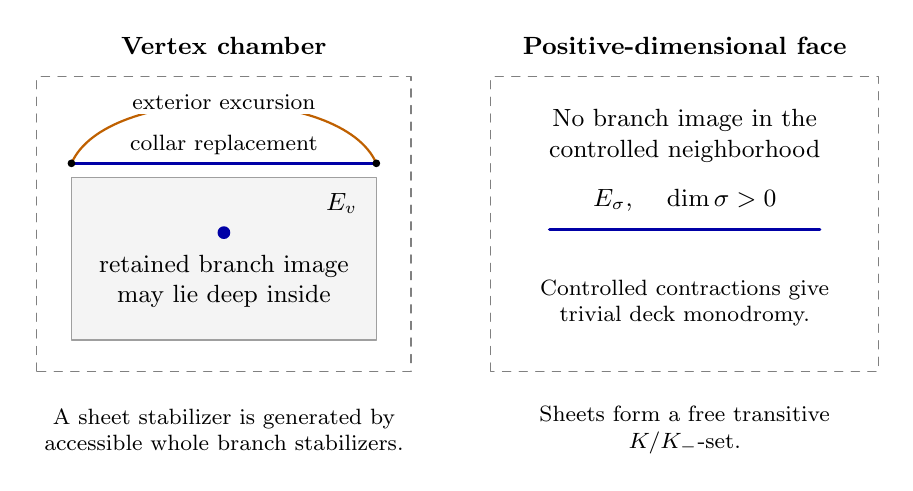
\begin{tikzpicture}[x=.88cm,y=.88cm,font=\small,
  every node/.style={align=center},line cap=round,line join=round]
  \node[font=\small\bfseries] at (2.8,5.35) {Vertex chamber};
  \draw[dashed,gray] (.1,.65) rectangle (5.5,4.9);
  \filldraw[fill=gray!9,draw=gray!75] (.6,1.1) rectangle (5,3.45);
  \node at (4.5,3.07) {$E_v$};
  \fill[blue!65!black] (2.8,2.65) circle (2.3pt);
  \node[text width=3.7cm] at (2.8,1.95)
    {retained branch image\\may lie deep inside};
  \draw[thick,orange!75!black]
    (.6,3.65) .. controls (1.1,4.8) and (4.5,4.8) .. (5,3.65);
  \node[font=\footnotesize,fill=white,inner sep=1.5pt] at (2.8,4.53)
    {exterior excursion};
  \draw[very thick,blue!65!black] (.6,3.65)--(5,3.65);
  \fill (.6,3.65) circle (1.4pt);
  \fill (5,3.65) circle (1.4pt);
  \node[font=\footnotesize,fill=white,inner sep=1pt] at (2.8,3.91)
    {collar replacement};
  \node[font=\footnotesize,text width=4.75cm] at (2.8,-.2)
    {A sheet stabilizer is generated by\\accessible whole branch stabilizers.};

  \node[font=\small\bfseries] at (9.45,5.35)
    {Positive-dimensional face};
  \draw[dashed,gray] (6.65,.65) rectangle (12.25,4.9);
  \node[text width=4.3cm] at (9.45,4.05)
    {No branch image in the\\controlled neighborhood};
  \draw[very thick,blue!65!black] (7.5,2.7)--(11.4,2.7);
  \node at (9.45,3.12) {$E_\sigma$, \quad $\dim\sigma>0$};
  \node[font=\footnotesize,text width=4.35cm] at (9.45,1.63)
    {Controlled contractions give\\trivial deck monodromy.};
  \node[font=\footnotesize,text width=4.85cm] at (9.45,-.2)
    {Sheets form a free transitive\\$K/K_-$-set.};
\end{tikzpicture}
\caption{Schematic coarse neighborhoods for selective cubulation. The
closed mid-halfspace chamber $E_v$ may contain retained branch images;
only the exterior collar used to shorten excursions must avoid them.
Every positive-dimensional face chamber $E_\sigma$ has a branch-free
controlled neighborhood. Consequently sheet transitions between
positive-dimensional faces are equivariant bijections, whereas vertex
sheet stabilizers may be nontrivial. The drawn regions and distances
are schematic: $E_v$ is not asserted to be the literal fiber
$p^{-1}(v)$, and the collar constants do not depend on chamber diameter.}
\label{fig:selective-chambers}
\end{figure}


Construct \(\widetilde Y\) by taking one copy of each cube of \(Y\) per
sheet of \(E_\sigma\), gluing along the face transitions.  These transitions
are compatible by construction, so this is a cubical complex, with
\begin{equation}
 q:\widetilde Y\longrightarrow Y
 \label{fill:cubical-cover}
\end{equation}
and an action of \(P\), inducing the \(\bar H\)-action downstairs.

\begin{lemma}[Cubical branched model]\label{fill:cubical}
The complex \(\widetilde Y\) is CAT(0), the \(P\)-action is cocompact,
and every hyperplane maps isomorphically under \(q\) to a hyperplane of
\(Y\).
\end{lemma}

\begin{proof}
First consider links.  Two adjacent lifted edge germs project to
distinct germs, since they occur on a cube projecting isomorphically
to a base cube.  Hence a clique projects to a clique with distinct germs.
An individual lifted edge determines a unique lift of every
positive-dimensional containing cube by the positive-face bijections
of Lemma~\ref{fill:sheets}.  The base flag condition and these bijections
therefore place all germs of the clique on its unique lifted cube.
Links are simplicial and flag.

We now establish simple connectivity; local flagness alone would not
suffice.  There is a useful canonical-lifting rule.  Suppose \(b\) maps
a path, disc, or homotopy into \(\widetilde X\), and \(a\) maps the same
parameter space into \(C\), with
\begin{equation}
 d\bigl(a,f\pi b\bigr)\le 2r+10r_0.
 \label{fill:close-maps}
\end{equation}
By the choice of \(D\), if \(p a\) lies in the open
cube \(\sigma\), the open-cube estimate in Lemma~\ref{fill:collapse}
assigns \(b\) to a sheet of \(E_\sigma\).  Use the corresponding copy of
\(\sigma\) to lift \(p a\).

This lift is continuous.  Near a parameter mapping into an open face,
local finiteness downstairs confines nearby values to cofaces of that
face.  Local path connectivity of the parameter space and the collar
assignment in Lemma~\ref{fill:sheets} make their sheet restrictions
agree on the face.  Although there can be infinitely many coface sheets
upstairs, their points approach this same face lift: distance to the
face is bounded by the corresponding coordinate distance inside a
unit cube, uniformly in dimension.  Thus the rule is continuous in
the cubical path metric.  In particular it applies to \(a=f\pi b\).

Conversely, let \(\alpha\) be an edge loop in \(\widetilde Y\), viewed
as a loop based at an edge midpoint.  For each of its edge occurrences
choose \(c_e\in E_e\) projecting to that midpoint, using the cube-lifting
assertion of Lemma~\ref{fill:collapse}.  Choose a nearby reference point
\(z_e\in\widetilde X\) in its assigned edge sheet.  Consecutive reference
points belong to the same vertex sheet, so join them by paths over the
\(r\)-neighborhood of the relevant \(E_v\).  These paths concatenate
to a loop \(b\) in \(\widetilde X\).

Project the image \(f\pi b\) piecewise to the convex sets \(E_v\),
adjusting its endpoints to the chosen \(c_e\)'s.  Nearest-point projection
and bounded endpoint interpolation give a homotopy satisfying
\eqref{fill:close-maps}.  Its canonical lift ends in paths lying in
closed half-stars of the prescribed lifted vertices.  To see this
precisely, a point of \(E_v\) has all outside-wall orientations equal
to those of \(v\), and every variable coordinate is at most halfway
from that corner.  Face consistency fixes the assigned lifted corner
throughout each path piece.  Straight-line contraction towards that
corner, compatible on faces, replaces the piece by the two required
half-edges.  The resulting loop is \(\alpha\).

Since \(\widetilde X\) is simply connected, \(b\) bounds a disc there.
The canonical lift for \(a=f\pi b\) maps this disc into
\(\widetilde Y\), proving that \(\alpha\) is nullhomotopic.
Every lifted vertex is also connected to the canonical image:
choose a reference point close to a lift of a base vertex in \(E_v\)
and use the same bounded interpolation.  Thus \(\widetilde Y\) is
connected and simply connected.  All cells have bounded finite shapes
and embedded faces; after subdivision, metric-open cell stars allow
ordinary fine-mesh simplicial approximation of the compact discs just
used.  Hence this argument proves the usual combinatorial simple
connectivity as well. Together with flag links it proves the CAT(0)
conclusion by \cite[Lecture~1, Section~1.2]{Sageev2014}.

The action is cocompact because \(Y/\bar H\) has finitely many cube
orbits and \(B\) is transitive on every sheet set.  Finally,
positive-dimensional face transitions make the restriction of \(q\)
to a hyperplane an ordinary covering of a base hyperplane.
Base hyperplanes are CAT(0), hence simply connected.  Each such
covering is therefore an isomorphism.
\end{proof}

\begin{proof}[Completion of Proposition~\ref{fill:selective}]
Take the finitely many hyperplane orbit families of the compact special
cover of \(C\), omitting families with no surviving members.  Within
each family hyperplanes are two-sided and disjoint.  These properties
pass to \(Y\): remaining walls do not acquire new crossings, by
Lemma~\ref{fill:collapse}.  They also pass to \(\widetilde Y\).

Cut successively along the lifts of each family, within the convex
components left by previous cuts.  Disjoint two-sided tracks in a
simply connected component give a tree splitting.  The resulting
graph-of-groups quotients are finite.  Indeed, subdivide along the
midplanes.  A chamber and its incident side pieces are specified by
cube-side flags up to the group action.  At a cell only the hyperplanes
cutting that cell can vary the choices of sides, so the number of
choices is bounded in terms of the dimension.  Branching at original
vertices introduces no additional midplane choices.

A cutting trace is a convex part of a lifted hyperplane.  It contains
a dual-edge midpoint in its chamber: in a cube meeting the trace, fix
the dual coordinate at its middle and choose the remaining corner
coordinates towards the chamber's defining sides.  Thus the trace
determines its containing hyperplane.  A deck transformation preserving
the trace preserves this hyperplane, acts trivially on it by
Lemma~\ref{fill:cubical}, and is trivial because positive-cell sheet
actions are free.  Hence the trace stabilizer injects into \(\bar H\).

The trace projects to a convex subcomplex of the corresponding base
hyperplane.  Each earlier cutting hyperplane meeting the lifted
hyperplane has a unique corresponding base trace; thus its side
condition projects to the same convex halfspace condition downstairs.
The stabilizer acts cocompactly on the trace by the finite flag
description.  Its image is consequently undistorted in \(Q_*\).
The quotient map \(P\to\bar H\) is Lipschitz in word metrics, so this
also proves undistortion of the trace stabilizer in the hyperbolic
group \(P\).  All edge groups of the hierarchy are therefore
quasiconvex in \(P\).

After all families are cut, each component has one original cubical
vertex.  Its stabilizer projects trivially to \(\bar H\), since
\(\bar H\) is torsion-free and acts properly on \(Y\).  It is exactly
the deck stabilizer of the corresponding vertex sheet.
Lemma~\ref{fill:sheets}(iii) says that this group is generated by
whole accessible retained factors, with finitely many factor orbits.
Apply Kurosh to its subgroup of
\[
 B=\mathop{*}_{a\ {\rm retained}}R_a.
\]
Each accessible whole factor is one of its Kurosh factors, up to
subgroup conjugacy.  Killing these factors kills the entire sheet
stabilizer by the proved generation statement.  Hence there can be
no remaining free summand or partial-factor summand.  The vertex
stabilizer is a finite free product of retained factors and is
hyperbolic and virtually compact special.

The hierarchy has finitely many levels and finite quotients.
Working upwards from its terminal groups shows that all vertex
groups are finitely generated.  The globally quasiconvex edge
groups give quasiconvex vertex groups successively: replace
excursions of an ambient path outside a vertex space by paths in
the attaching edge cosets, using their ambient undistortion.
The quasiconvex hierarchy theorem \cite{Wise2021} therefore makes
\(P\) virtually compact special.  The normal-core choice made above
establishes the asserted normality of \(H\), and any later normal
core can be accommodated by repeating the same sparse-cover
construction.
\end{proof}

\subsection{Novikov realization along quotient chains}

The geometric construction now supplies quotients that retain any
prescribed finite set of filling-kernel factors. Our algebraic target is
to realize any finite list of rational expressions, after finite-index
restriction, in the ordinary Novikov rings for both signs of one real
character. Applied to the entries of a division-ring chain contraction,
this will give the two acyclicity statements needed for fibering.
We first descend through an RFRS chain of the quotient until the
remaining coefficients lie in \(D(K)\). A selective quotient then
makes their finitely many subgroup supports detectable by a second
RFRS chain. That descent ends with ordinary group-ring coefficients;
recombination recovers the original expressions for one character and
its negative.

For a real character \(\chi:J\to\R\), write
\begin{equation}
 \widehat{\Q J}^{\,\chi}
 =\left\{\sum_{g\in J}a_g g:
       \#\{g:a_g\ne0,\ \chi(g)<c\}<\infty
       \text{ for every }c\in\R\right\}.
 \label{fill:novikov-ring}
\end{equation}
Our completion convention is towards positive height.
The subgroup-field hypotheses embed \(D(J)\) and this ring in the same
skew series division ring over \(D(\ker\chi)\).  Indeed,
\eqref{fill:field} embeds the rational field there; a nonzero series
has a leading term, and its positive remainder has a positive minimum
valuation, so geometric inversion is defined.  This remains valid when
\(\chi(J)\) is dense in \(\R\), because the support condition is finite
below each threshold.

\begin{definition}\label{fill:selective-input}
Let \(K\lhd J\), with \(J/K\) virtually RFRS.
We say that \((J,K)\) has the \emph{selective realization property} if,
for every finite-index preimage \(J'\le J\) and every finite set
\(T\subset K\), there are a finite-index preimage \(H\le J'\), normal
in \(J'\), a subgroup \(U\le K\) containing \(T\), and a homomorphism
from \(H\) to a virtually RFRS group that is injective on \(U\).
\end{definition}

Proposition~\ref{fill:selective} supplies this property in
Theorem~\ref{fill:criterion}: a finite set in \(K\) lies in a finite
subproduct of \eqref{fill:CL}, and its selective quotient is virtually
compact special, hence virtually RFRS \cite{Agol2008}.
More explicitly, let \(\rho:H\to L\) be the selective homomorphism
and let \(S\) be a finite transversal for \(H\backslash J'\).
Normality of \(H\) makes
\[
 h\longmapsto\bigl(\rho(s^{-1}hs)\bigr)_{s\in S}
 \qquad(h\in H)
\]
a homomorphism on the common domain \(H\). Its \(s\)-coordinate is
injective on \(sUs^{-1}\). These are the conjugate support groups
arising in the right-coset coordinates for restriction of scalars.
Finite products
and subgroups of RFRS groups are RFRS, so the product target remains
virtually RFRS.

\begin{lemma}[Controlled linearization]\label{fill:linearize}
A rational expression over a coefficient ring in a division ring has
a representation \(pA^{-1}q\), where \(A\) is a square polynomial
matrix and \(p,q\) are constant selectors.  The entries of \(A^{-1}\)
can be given rational expressions using sums and products of the
original subexpressions and their original inverses.  In particular
linearization introduces neither a larger nested inverse depth nor
new bottom denominators on a maximal-depth inverse chain.
\end{lemma}

\begin{proof}
A polynomial \(f\) is the upper-right entry of the inverse of
\(\begin{psmallmatrix}1&-f\\0&1\end{psmallmatrix}\).
Use block diagonals for sums.  If \(E=pA^{-1}q\) and \(F=rB^{-1}s\),
use
\[
 \begin{pmatrix}A&-qr\\0&B\end{pmatrix}^{-1}
 =
 \begin{pmatrix}
 A^{-1}&A^{-1}qrB^{-1}\\0&B^{-1}
 \end{pmatrix}
\]
for the product.  For \(E^{-1}\), border \(A\) to obtain
\begin{equation}
 M=\begin{pmatrix}0&p\\q&A\end{pmatrix},\qquad
 M^{-1}=
 \begin{pmatrix}
 -E^{-1}&E^{-1}pA^{-1}\\
 A^{-1}qE^{-1}&A^{-1}-A^{-1}qE^{-1}pA^{-1}
 \end{pmatrix}.
 \label{fill:border}
\end{equation}
The displayed formulas prove the assertion inductively.  In
\eqref{fill:border} the new inverse is exactly the parent inverse
already present in the original expression.
\end{proof}

The data at a descent stage are finitely many square polynomial
matrices invertible over the current division ring, together with
chosen rational expressions for all entries of their inverses.
Linearization puts a finite list of scalar expressions in this form.
Truncating a character expansion records finitely many coefficient
entries. Solving those coefficient problems means realizing their
chosen rational values in both ordinary Novikov rings for one later
character. The next lemma proves that this reduction terminates;
the following lemma explains how to recover the original inverses.

\begin{lemma}[Finite descent of inverse depth]\label{fill:ancestry}
Let \(J/K\) have a normal RFRS chain, and pull it back to
\[
 J=H_0\ge H_1\ge\cdots,\qquad \bigcap_iH_i=K.
\]
Let \(N_i\lhd H_0\) be the preimage of the rational abelianization
kernel of \(H_i/K\), so \(N_i\le H_{i+1}\).
At each stage expand finitely many specified rational expressions
for both signs of a character with kernel \(N_i\), retain finitely
many coefficients, restrict those scalar coefficient problems to
\(H_{i+1}\), and use Lemma~\ref{fill:linearize}.
After finitely many stages the resulting coefficient problems have
inverse depth zero over \(D(K)\).
\end{lemma}

\begin{proof}
Inverse depth is measured relative to \(D(K)\): coefficient-field
elements and group monomials have depth zero, sums and products
take the maximum, and inversion adds one.  At the bottom of an
inverse chain, evaluate the inverse-free operand as a finite
polynomial before taking slices.

For one character, write an operand with leading monomial \(L\) as
\(L(1+T)\), with \(T\) of strictly positive valuation.  Its inverse
is \(\sum_{n\ge0}(-T)^nL^{-1}\).  Every specified coefficient is a
finite sum of products of operand coefficients, monomial transports,
and the inverse of the leading coefficient.  Thus depth does not
increase.

There is a more precise invariant.  If a coefficient retains the
old maximum depth \(d>0\), each bottom denominator on a length-\(d\)
inverse chain is a height slice of an old bottom polynomial on a
length-\(d\) chain, up to common monomial transport and conjugation.
For sums and products the assertion follows by tracing a
maximal-depth chain into one factor.  For an inverse, coefficients
of its operand alone have depth at most \(d-1\).  A chain of length
\(d\) must therefore pass through the inverse of the leading
coefficient.  Apply the same induction to that coefficient of the
operand.  At the bottom this is simply a slice of an inverse-free
polynomial.  Cancellations remove terms but introduce no new support
degree in that bottom polynomial.

Choose one right normalizing monomial for each slice.  Replacing
support elements \(g,h\) by \(gu^{-1},hu^{-1}\) leaves \(gh^{-1}\)
unchanged.  A later whole conjugation conjugates this ratio.
Consequently, while depth \(d\) persists, the nonidentity differences
of its bottom support degrees modulo \(K\) lie among conjugates of
a fixed finite list, chosen at the beginning of this depth block.

Restriction to the next subgroup does not mix the coefficients:
for \(c\in D(N_i)\) and a representative \(t\) of
\(H_{i+1}\backslash H_i\),
\begin{equation}
 t c=(tct^{-1})t,\qquad tct^{-1}\in D(N_i)\subset D(H_{i+1}).
 \label{fill:diagonal}
\end{equation}
Thus the coefficient operator is diagonal by conjugation on these
coset coordinates.  Controlled linearization also preserves the
invariant by Lemma~\ref{fill:linearize}.

The bottom support differences at stage \(i\) belong to \(H_i/K\).
Since these subgroups are normal and have trivial intersection,
eventually they exclude every element of the fixed finite list and
all its conjugates.  Every bottom operand on a surviving maximal-depth
chain is then a monomial over \(D(K)\).  Inverting it uses only a
monomial inverse and a coefficient-field inverse, so all such chains
shorten.  Start a new finite list after this depth drop and repeat.
There are finitely many depth drops.

The qualification about maximal depth is essential to this argument.
New denominator supports can appear after the depth drops; the
construction expressly starts a fresh finite list at that point.
It never asserts that one support list controls all later depths.
\end{proof}

A given RFRS chain may be replaced by one normal in its initial group.
Indeed, intersect its finitely many conjugates at each stage; the
rational abelianization kernel of a subgroup maps into that kernel
in every containing conjugate.  The RFRS containment therefore
persists under these cores. In the finitely generated setting of
Proposition~\ref{fill:progressive}, characters with kernel exactly
\(N_i\) exist by embedding the finite-rank free abelian group
\(H_i/N_i\) in \(\R\). A zero character is permitted at a stationary
stage. Depth zero over \(D(K)\) still allows coefficients in that
division ring: it need not mean a polynomial over \(\Q K\). Removing
precisely those remaining coefficients will require the selective
realization property.

\begin{lemma}[Recombination by perturbation]\label{fill:recombine}
Suppose a finite stage of the preceding procedure used a character
\(\chi_i\) on \(H_i\). For each of its polynomial matrices \(A\), fix
finite homogeneous truncations \(B_+,B_-\) of \(A^{-1}\) such that
\(I-AB_\pm\) and \(I-B_\pm A\) have strictly positive weights for
\(\pm\chi_i\), respectively. Suppose all scalar coefficients of the
matrices \(A,B_+,B_-\) have been realized, after restriction to a
finite-index subgroup \(F\), in both ordinary Novikov rings for a
character \(\psi\) of \(F\), compatibly with their rational-field values.
Then its original matrix inverse problems are realized for both
signs of
\begin{equation}
 \chi_i|_F+\epsilon\psi
 \label{fill:perturb}
\end{equation}
for every sufficiently small positive \(\epsilon\).
\end{lemma}

\begin{proof}
Let \(A\) be one polynomial matrix and \(B=A^{-1}\), with its
specified rational expressions. The chosen truncations \(B_+\) and
\(B_-\) have coefficients in \(D(N_i)\), and both errors
\begin{equation}
 I-AB_\pm,\qquad I-B_\pm A
 \label{fill:errors}
\end{equation}
have strictly positive weights in their respective directions.

First we check the support needed to compare the two characters.
This is necessary even when a later finite-index cut does not
contain \(N_i\).
For right-coset coordinates \(t_j\) of \(F\backslash H_i\), the
entry from \(t_j\) to \(t_k\) of a homogeneous term of degree \(u\)
is supported in the single height
\begin{equation}
 u+\chi_i(t_j)-\chi_i(t_k).
 \label{fill:offset}
\end{equation}
Its coefficient lies in one coset of \(D(F\cap N_i)\): use the
finite-index field decomposition on the intersection of its original
homogeneous coset with the selected matrix coset. Put \(U=F\cap N_i\)
and first remove this common monomial shift. Choose a finitely generated
subgroup of \(U\) supporting a rational expression for the remaining
coefficient, and expand there for the restriction of \(\psi\).
Uniqueness of rational inverses in the ambient skew-series ring
identifies this intrinsic expansion with the ambient one. At each
\(\psi\)-height an ordinary Novikov realization has only finitely many
group terms. Subgroup-coset independence applied to that finite
coefficient sum excludes terms outside \(U\). Multiplying back by the
common shift proves preservation of the original homogeneous support.
The same argument applies across the selective change of quotient,
where the support subgroup embeds.

On \(F\cap N_i\), the new character in \eqref{fill:perturb} is
\(\epsilon\psi\).  The internal series expansion is therefore
unchanged, with only its grading scaled; it represents the same
rational entry.  Every finite old-height slice remains summable.
For each sign, subtract the row-minus-column offsets in
\eqref{fill:offset} when measuring an error entry.
There are finitely many positive old-height slices, and their
\(\pm\psi\)-valuations are bounded below.  A common sufficiently
small positive \(\epsilon\) therefore keeps all adjusted error
valuations strictly positive.

Offsets telescope in matrix products.  Hence powers of either
error in \eqref{fill:errors} have valuations tending to positive
infinity, even in the unadjusted coordinates.  Geometric inversion
provides both a left and a right inverse for \(A\) in the relevant
ordinary Novikov ring; they coincide.  All identities are exact
because the rational field and the ordinary series were embedded
in the same skew series division ring.  The same choice of
\(\epsilon\) works for the finite lists for both signs.
\end{proof}

\begin{proposition}[Progressive characters]\label{fill:progressive}
Let \(J\) be finitely generated with the subgroup-field hypotheses,
and let \(K\lhd J\) satisfy the selective realization property of
Definition~\ref{fill:selective-input}.
Every finite family of rational expressions over \(\Q J\) can,
after restriction of scalars to a finite-index subgroup \(F\),
be realized compatibly in the ordinary Novikov rings for both signs
of a single real character of \(F\).

In particular, if a finite complex of finitely generated free
\(\Q J\)-modules is acyclic over \(D(J)\), then its restriction is
acyclic over both these Novikov rings.  If its degree-zero ordinary
homology is nonzero, the character is nonzero.
\end{proposition}

\begin{proof}
Take the preimage \(H_0\) of a finite-index RFRS subgroup of \(J/K\).
Restriction of scalars is right multiplication on right-coset
coordinates, using a normal core when necessary.  The finite-index
field decomposition makes this an exact finite matrix operation.
Linearize the finitely many expressions as in
Lemma~\ref{fill:linearize}, retaining the specified expressions for
all needed inverse entries.

Pull back a normal RFRS chain from \(H_0/K\).  At stage \(i\), use
\eqref{fill:field} to expand each inverse matrix for both signs of
a character \(\chi_i\) with kernel \(N_i\).  Truncate sufficiently
far to obtain the positive errors \eqref{fill:errors}.  Collect
the finitely many coefficients of the matrix and its truncations;
they lie in \(D(N_i)\).  Restrict to the next group by
\eqref{fill:diagonal}, and linearize these scalar problems.
Lemma~\ref{fill:ancestry} terminates this procedure with finitely
many unresolved coefficients in \(D(K)\).

Choose a finite set of elements of \(K\) supporting rational
expressions for all those coefficients.  Apply the selective
realization property, including its finite product of conjugate
maps, to obtain a normal finite-index preimage \(H\) and a map
injective on the required support subgroups.  Pass to the
preimage \(H_p\) of an RFRS subgroup of its image.

This cut can mix coefficient entries, so we describe it explicitly.
For a scalar \(c\in D(U_0)\), group the cosets of \(H_p\) into
orbits of right multiplication by \(U_0\).  An orbit has
representatives \(gu_j\), with \(u_j\in U_0\).
The entries of right multiplication by \(c\) in these coordinates
come from decomposing \(u_jc\) over
\[
 D(U_0\cap g^{-1}H_p g)
\]
and then conjugating by \(g\).  They therefore admit finite rational
expressions entirely in these subgroup fields.
Changing to one common transversal only multiplies entries by
monomials, which does not affect summability.

Start the depth argument afresh with these new expressions.
Use an RFRS chain in the new quotient and ordinary rational group
polynomials.  Work separately inside each support subgroup,
choosing its own monomial transporters when taking a height
coefficient.  Later coefficients remain in conjugates of that
support subgroup.  Once a coefficient lies in the current
character kernel, restriction to the next stage only conjugates
it, because that whole kernel is contained in the next subgroup.
Thus the maximal-depth ancestry argument applies exactly as
before.  The new quotient map is injective on each support subgroup,
so its normal RFRS chain separates the finite nonidentity support
lists.  This time the terminal problems are ordinary group-ring
polynomials, with no unresolved division-field coefficients.
They are realized for the zero character if necessary.

Now reconstruct the inverse problems backwards, through both
finite chains and the selective switch, using
Lemma~\ref{fill:recombine}.  At each step use both signs' residual
lists and choose one sufficiently small positive perturbation.
The result is a single character on a common finite-index subgroup
and compatible realizations of all original expressions for both
of its signs.

For the chain-complex assertion, include the entries of a
\(D(J)\)-chain contraction and all the inverse operands used in
their expressions.  Their exact identities persist under the
common series embeddings, giving contractions over the two
ordinary Novikov rings. Restriction of scalars does not change the
underlying chain complex or its ordinary homology. If the final
character were zero, its Novikov rings would be \(\Q F\), so these
contractions would contradict the assumed nonzero ordinary
degree-zero homology.
\end{proof}

\begin{corollary}[Open Novikov regions for RFRS groups]\label{fill:rfrs-novikov}
Let \(J\) be virtually RFRS with the subgroup-field hypotheses.
A finite family of bounded complexes of finitely generated free
\(\Q J\)-modules, with polynomial differential matrices and acyclic
extension to \(D(J)\), admits simultaneous ordinary Novikov contractions,
after passage to a finite-index subgroup \(F\), on a nonempty
antipodally invariant open subset of \(\Hom(F,\R)\).
Here the character space has the topology of pointwise convergence.
This property can be imposed after any prescribed further finite-index
restriction.
\end{corollary}

\begin{proof}
We use the descent above with \(K=1\), so there is no selective
switch. For finitely generated \(J\), the underlying realization is
also supplied by \cite[Theorem~5.2]{Kielak2020}. To retain the present
group generality, we first justify the ambient characters and the
character-field expansion without finite generation.

Choose a finite-index RFRS subgroup \(H_0\) and a normal residual
chain \((H_i)\). The embedding
\(H_0\hookrightarrow\prod_i H_0/H_i\) into a countable product of
finite groups gives \(|H_0|\leq|\R|\). If \(N_i\) is the rational
abelianization kernel of \(H_i\), the rational hull of the torsion-free
abelian group \(H_i/N_i\) therefore has dimension at most
\(\dim_{\Q}\R\). A rational-linear injection into \(\R\) supplies
a character of the whole group \(H_i\) with kernel exactly \(N_i\).
The quotient need not be free abelian or finitely generated. The
RFRS containment \(N_i\leq H_{i+1}\) still holds.

For any real character \(\chi\) of a subgroup \(H\), put
\(N=\ker\chi\). Coset independence embeds
\(D(N)*(H/N)\) in \(D(H)\). This crossed product is the directed
union of its subrings over finitely generated subgroups of \(H/N\).
Each such subgroup is free abelian of finite rank, and its crossed
product is an iterated skew Laurent Ore domain. Every pair of
elements lies in one such subring, where its left and right Ore
equations can be solved. The union is therefore Ore as well.
Its fraction division ring embeds in \(D(H)\), since \(D(N)\), the
group lifts and all inverses of nonzero elements lie there. Conversely,
the fraction ring contains \(\Q H\), so it contains its division
closure \(D(H)\). The fraction ring is thus exactly \(D(H)\),
proving \eqref{fill:field} in this generality.

The same skew-series realization applies: a nonempty support finite
below every real threshold has a least term, and each strictly positive
remainder has an individual positive minimum valuation. These facts
justify geometric inversion even when the character image is dense
or not finitely generated.

Start with the finitely many entries of division-ring chain
contractions. The descent in Lemma~\ref{fill:ancestry} uses only finite
rational expressions, finite retained coefficient lists and finite-index
transversals. Normal residuality removes its finite support-difference
lists, so it terminates with coefficients over \(D(1)=\Q\).
Lemma~\ref{fill:recombine} then applies backwards: there are finitely
many old-height slices and lower bounds for their later-character
valuations, so one positive perturbation works for both signs at each
stage. This gives simultaneous ordinary Novikov contractions.

For openness, linearize the finitely many contraction entries over
the ordinary group ring and truncate their realized inverse matrices
to finite group-ring matrices. The left and right inverse errors have
finitely supported strictly positive valuations. Their finitely many
strict evaluation inequalities define an open neighborhood in the
pointwise topology, and geometric inversion supplies the contractions
throughout it. Intersect the neighborhood for the positive sign with
the negative of the neighborhood for the negative sign, and then take
the union with its negative. This is the required nonempty antipodally
invariant open set.

On restriction to any deeper finite-index subgroup, a Novikov
series remains summable in its finite coset coordinates, with
only fixed monomial offsets.  Repeat the finite truncation
argument there to obtain openness in the larger character space.
\end{proof}

\subsection{From two-sided Novikov acyclicity to a free kernel}

\begin{lemma}[The degree-one Novikov implication]\label{fill:bns}
Let \(J\) be finitely presented, and let \(\chi:J\to\R\) be nonzero.
If degree-one homology vanishes over
\(\widehat{\Q J}^{\,\chi}\), then \(\chi\) belongs to the Bieri--Neumann--Strebel (BNS)
invariant.  If the vanishing holds for both signs, some nonzero
rational character has finitely generated kernel.
\end{lemma}

\begin{proof}
We include the rational-coefficient argument in the positive-completion
convention of \cite[Theorem~3.11]{Kielak2020}; Sikorav established the
integral-coefficient criterion \cite{Sikorav1987}.
Choose a symmetric generating set containing a generator \(t\)
with \(\chi(t)>0\).  In the positive completion the formal ray
\[
 c=\sum_{j\ge0}[t^j,t^{j+1}]
\]
has boundary \(-[1]\).  For each oriented generator \(x\), the
chain
\[
 [1,x]+xc-c
\]
is a cycle, hence bounds a completed rational two-chain in the
finite presentation complex.

Truncate that two-chain sufficiently high.  Since relators have
bounded height offsets, its boundary cancels every low term of
the displayed cycle.  Truncate both rays at a common sufficiently
large exponent \(k\).  The resulting finite one-chain can be
made to have arbitrarily high support and boundary
\[
 [xt^k]-[t^k].
\]
The component of its edge support containing one endpoint must
contain the other: the total boundary coefficient in a finite
connected component is zero.  Thus \(t^k\) and \(xt^k\) are joined
by an actual path at uniformly high height, for every generator
\(x\).

Translate these finitely many paths to replace each edge
\(g\to gx\) by a path from \(gt^k\) to \(gxt^k\).
Choose the height threshold so this replacement raises the
minimum height by a fixed positive amount.  Iterating pushes
any finite path above height zero.  Its original nonnegative
endpoints are connected to their pushed copies by positive
\(t\)-rays, so the nonnegative Cayley graph is connected.
This is the BNS condition.

The finite paths and their strict height inequalities persist
in a neighborhood of \(\chi\).  Applying the same construction
to \(-\chi\) gives both BNS conditions on a nearby nonzero
rational line.  The two-sided BNS criterion
\cite[Theorem~B1]{BNS1987}, also stated in
\cite[Theorem~3.10]{Kielak2020}, says that the kernel of its integral representative
is finitely generated.
\end{proof}

\begin{lemma}[A finitely presented kernel in dimension two]\label{fill:free-kernel}
Suppose \(\cd J\le2\) and \(J\) maps onto \(\Z\) with finitely
presented kernel \(M\).  Then \(M\) is free.
\end{lemma}

\begin{proof}
We have \(\cd M\le2\).  If \(\cd M=2\), finite presentation gives
a finite-length resolution of \(\Z\) by finitely generated
projective \(\Z M\)-modules, with the last module in degree two.
Its dual has nonzero degree-two cohomology:
otherwise its last map would split, and dualizing back would
shorten the original projective resolution.  Thus
\[
 H^2(M;\Z M)\ne0.
\]

As an \(M\)-module, \(\Z J\) is a direct sum of copies of \(\Z M\)
indexed by \(J/M=\Z\).  Finite generation of the resolution gives
the corresponding direct-sum description of \(H^2(M;\Z J)\).
The generator of \(J/M\) shifts the summands, with its conjugation
twist.  Its coinvariants are therefore nonzero.  The
Lyndon--Hochschild--Serre cohomology spectral sequence has only columns
zero and one for this quotient, so
\[
 H^3(J;\Z J)
 \cong H^1\bigl(\Z;H^2(M;\Z J)\bigr)\ne0,
\]
contrary to \(\cd J\le2\); see \cite{Brown1982,Bieri1976}.
It follows that \(\cd M\le1\), and Stallings--Swan
\cite{Stallings1968,Swan1969} makes \(M\) free.
\end{proof}

\begin{proof}[Proof of Theorem~\ref{fill:criterion}]
First suppose \(G_*\) is already VCS, as happens when the peripheral
family is empty after discarding trivial members or contains \(G_*\)
itself. Then \(G_*\) is virtually RFRS, so
Corollary~\ref{fill:rfrs-novikov} applies directly to its finite
classifying-space chains. This gives two-sided Novikov contractions
on a finite-index subgroup \(F\), without using the filling construction.

In the remaining case choose the cofinite good filling
\eqref{fill:cofinite}. Proposition~\ref{fill:selective} gives the
selective realization property, and Proposition~\ref{fill:progressive}
applied to the same chains again supplies two-sided Novikov
contractions on a finite-index subgroup \(F\).

In either case the restricted group-ring chain complex has
\(H_0\cong\Q\): it is the cellular complex of the same connected
universal cover, now with the \(F\)-action. The character cannot be
zero, since its Novikov ring would then be \(\Q F\), and a contraction
would contradict this ordinary \(H_0\). Lemma~\ref{fill:bns} therefore
gives a nonzero rational character on \(F\) with finitely generated
kernel. Rescaling its image gives an epimorphism \(F\to\Z\).

Coherence makes this kernel finitely presented.
Lemma~\ref{fill:free-kernel} makes it free, and finite generation
makes its rank finite.  The extension splits by choosing a lift
of a generator of \(\Z\), so the subgroup is finite-rank
free-by-cyclic.  It is hyperbolic, hence admits a proper cocompact
cubulation by \cite{HagenWise2016}; the elementary rank-zero case
is immediate.  Agol's theorem \cite{Agol2013} now gives virtual
compact specialness, which passes to the finite-index overgroup
\(G_*\).
\end{proof}
